\documentclass[a4paper,11pt]{article}
\usepackage[T2A]{fontenc}     
\usepackage[utf8]{inputenc}  
\usepackage{lmodern}  
\usepackage{amsmath}
\usepackage{amsfonts}
\usepackage{amssymb} 
\usepackage{listings}
\usepackage{lstcustom}
\usepackage{graphicx}
\usepackage{pstricks}
\usepackage{geometry} % Меняем поля страницы
\geometry{left=2cm}% левое поле
\geometry{right=1.5cm}% правое поле
\geometry{top=1cm}% верхнее поле
\geometry{bottom=2cm}% нижнее поле
\renewcommand\lstlistingname{Листинг}
\renewcommand\contentsname{Содержание}
\renewcommand\partname{ }
\renewcommand{\thepart}{\arabic{part}}


\title{Лабораторная работа №4. Решение систем линейных алгебраических уравнений с помощью метода квадратного корня}
\author{Архангельский Илья}


\begin{document}
\begin{titlepage}
	\begin{center}
		БЕЛОРУССКИЙ ГОСУДАРСТВЕННЫЙ УНИВЕРСИТЕТ \\
		ФАКУЛЬТЕТ ПРИКЛАДНОЙ МАТЕМАТИКИ И ИНФОРМАТИКИ
	\end{center}
	\vspace{10em}
	\begin{center}
		\LARGE {Лабораторная работа \\
		по вычислительным методам алгебры на тему:}
		\linebreak	 
		
    Решение систем линейных алгебраических уравнений с помощью метода квадратного корня
	\end{center}
	\vspace{3em}
	\begin{flushright}
	  
	
 	Выполнил: \\	Архангельский И.А. \\ 
 	
 	  \vspace{1em}
 	
 	  Проверил: \\ Кондратюк А.П. \\
 	
	\end{flushright}
	
	\vfill
	\begin{center}
		Минск, 2012
	\end{center}
\end{titlepage} 

\newpage
\part*{Входные и выходные данные.} 
\section*{Входные данные}
Входной файл в первой строке содержит число $n$ - размерность матрицы коэффициентов, следующие $n$ строк содержат матрицу $(A|f)$, где  
  $A$ - квадратная матрица коэффициентов СЛУ, 
  $f$ - вектор-столбец свободных членов.
\section*{Выходные данные}
На выход в stdout подается решение системы если оно существует, в случае, если систему решить невозмножно выводится DivByZero. 
\newpage
\part*{Блок-схема} 
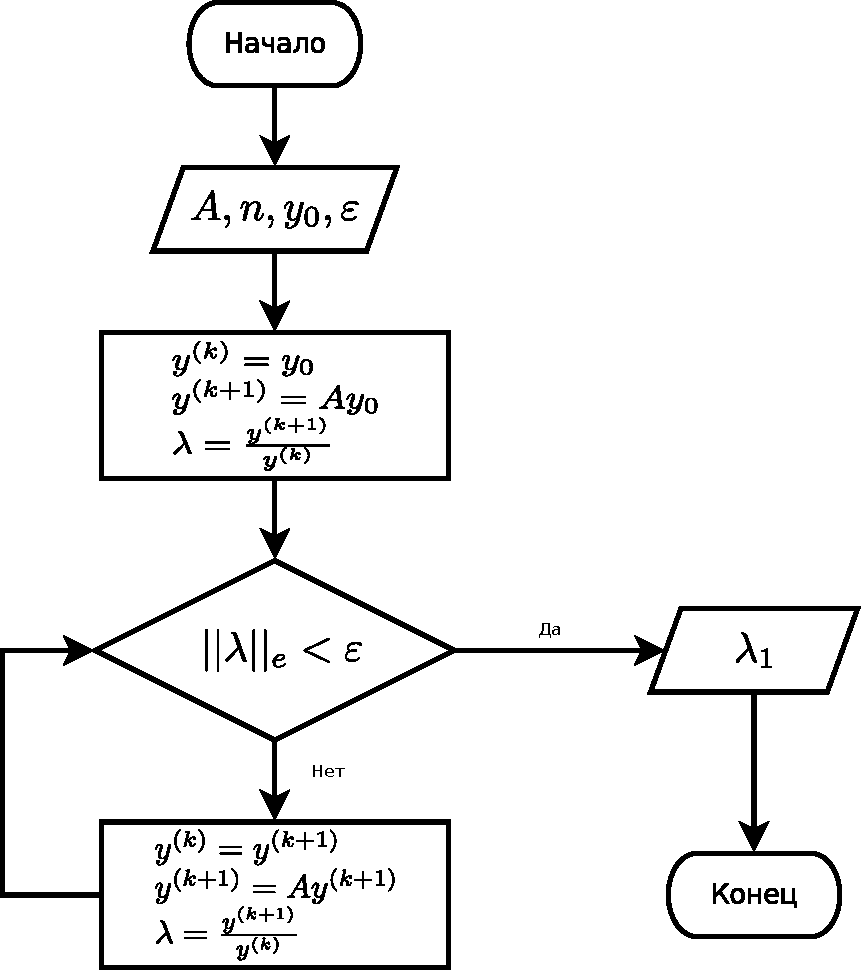
\includegraphics[scale=0.85]{flowchart.pdf}
 


\newpage
\part*{Реализация}
\lstinputlisting[language=C++, style=eclipse, basicstyle=\scriptsize, title={square.h}]{"../Square/square.h"}
 
\lstinputlisting[language=C++, style=eclipse, basicstyle=\scriptsize, title={square.cpp}]{"../Square/square.cpp"}
 
\lstinputlisting[language=C++, style=eclipse, basicstyle=\scriptsize, title={main.cpp}]{"../Square/main.cpp"}
 
 \newpage
\part*{Тестовые данные}
\begin{footnotesize}
\framebox{
  \begin{minipage}[t]{0.4\linewidth}   
  \lstinputlisting[title={test01.in}]{"../tests/test01.in"}
  \end{minipage}
  \begin{minipage}[t]{0.6\linewidth}
  \lstinputlisting[title={test01.out}]{"../tests/test01.out"}
  \end{minipage}
}
\framebox
{ 
  \begin{minipage}[t]{0.4\linewidth}   
  \lstinputlisting[title={test02.in}]{"../tests/test02.in"}
  \end{minipage}
  \begin{minipage}[t]{0.6\linewidth}
  \lstinputlisting[title={test02.out}]{"../tests/test02.out"}
  \end{minipage}
}
\framebox
{
  \begin{minipage}[t]{0.4\linewidth}
  \lstinputlisting[title={test03.in}]{"../tests/test03.in"}
  \end{minipage}
  \begin{minipage}[t]{0.6\linewidth}
  \lstinputlisting[title={test03.out}]{"../tests/test03.out"}
  \end{minipage}  
}
\framebox
{
  \begin{minipage}[t]{0.4\linewidth}
  \lstinputlisting[title={test04.in}]{"../tests/test04.in"}
  \end{minipage}
  \begin{minipage}[t]{0.6\linewidth}
  \lstinputlisting[title={test04.out}]{"../tests/test04.out"}
  \end{minipage}
}
\framebox
{
  \begin{minipage}[t]{0.4\linewidth}
  \lstinputlisting[title={test05.in}]{"../tests/test05.in"}
  \end{minipage}
  \begin{minipage}[t]{0.6\linewidth}
  \lstinputlisting[title={test05.out}]{"../tests/test05.out"}
  \end{minipage}  
}
\end{footnotesize}
\end{document}
